\documentclass[10pt,xcolor={usenames,dvipsnames,table},aspectratio=169]{beamer}
\usepackage{tri_preamble}

%----------------------------------------------------------------------------------------
%	TITLE PAGE
%----------------------------------------------------------------------------------------

\title[Fano's method]{Minimax lower bound: Fano's method} 

\author{Tri Nguyen} 
\institute[OSU] 
{
    Reading group - Summer 2022 \\
Oregon State University 
% \medskip
% \textit{nguyetr9@oregonstate.edu \endgraf } 
% }
}
\date{\today} % Date, can be changed to a custom date


\makeatletter
\makeatother


\begin{document}

\frame{\titlepage}


\begin{frame}
    \frametitle{Let's start with an example}
    \begin{itemize}
        \item Given a family of Gaussian $\mathcal{N}_d = \set{N(\theta, \sigma^2 I_d) | \theta \in \mathbb{R}^{d}}$.
        \item God chooses a distribution $P \in \mathcal{N}_d$.
        \item A set of $n$ i.i.d samples are drawn from  $P$. 
        \item Task: estimate the mean $\theta$ from $n$ samples.
        \item Quality of estimator is measured by $ \mathbb{E}\left[  \norm{\theta - \widehat{\theta}}^2\right]$
    \end{itemize}
What could be the best performance in the worse case scenario?
\begin{itemize}
    \item If $d=1$, we can use Cramer-Rao lower bound.
    \item Sample mean estimator have the error of  $\dfrac{d\sigma^2}{n}$, let's see if this error can be improved.
\end{itemize}
\end{frame}


\begin{frame}
    \frametitle{Setting}
    \begin{itemize}
        \item From a distribution family $\mathcal{P}$, God chooses a distribution $P \in \mathcal{P}$.
        \item A set of $n$ i.i.d samples $X_1^{n}$ are drawn from  $P$.
        \item Task: estimating $\theta(P)$ from given samples.
        \item Question: What would be the best performance of an ideal estimator in the worse case?
        \item Quality of estimator is measured by $\Phi(\rho(\theta, \widehat{\theta}))$, where:
            \begin{itemize}
                \item $\phi := \phi(P)$  is some statistic of $P$
                \item  $\widehat{\theta}:=\widehat{\theta}(X_1^{n})$ is some estimator
                \item $\Phi(\cdot)$ is a non-decreasing function
                \item $\rho(\cdot, \cdot)$ is a semimetric
            \end{itemize}
    \end{itemize}
    \[
    \mathcal{M}_n(\theta(\mathcal{P}), \Phi \circ \rho) := \inf_{\widehat{\theta}} \sup_{P \in \mathcal{P}} \mathbb{E} \left[  \Phi(\rho(\theta, \widehat{\theta})) \right]
    \] 
    Finding exact $\mathcal{M}()$ is difficult, instead our attempt is to find a lower bound of it.
\end{frame}

\begin{frame}
\frametitle{Sketch}   

    \[
    \mathcal{M}_n(\theta(\mathcal{P}), \Phi \circ \rho) := \inf_{\widehat{\theta}} \sup_{P \in \mathcal{P}} \mathbb{E} \left[  \Phi(\rho(\theta, \widehat{\theta})) \right]
    \] 
    \begin{enumerate}
        \item Translate to probability
            \[
            \inf_{\widehat{\theta}} \sup_{P \in \mathcal{P}} \mathbb{E} \left[  \Phi(\rho(\theta, \widehat{\theta})) \right]
            \geq \Phi(\delta) \inf_{\widehat{\theta}} \sup_{P \in \mathcal{P}} \mathbb{P}(\rho(\theta, \widehat{\theta}) \geq \delta)
            \] 
        \item Reduce the whole space $ \mathcal{P}$ to a finite set $\set{\theta_v| v \in \mathcal{V}}$
            \[
            \sup_{P \in \mathcal{P}} \sum_{v \in \mathcal{V}} \mathbb{P}(\rho(\theta, \widehat{\theta}) \geq \delta) \geq \dfrac{1}{\abs{\mathcal{V}}} \mathbb{P}(\rho(\theta_v, \widehat{\theta}) \geq \delta)
            \] 
        \item Reduce to a hypothesis testing error (required $\mathcal{V}$ to have some properties)
            \[
            \mathbb{P}(\rho(\theta_v, \widehat{\theta}) \geq \delta) \geq \mathbb{P}(\Psi(X_1^{n}) \neq v)
            \] 
        \item Finding concrete bound based on specific problems.

    \end{enumerate}
\end{frame}

\begin{frame}
    % \begin{itemize}
        % \item A $\delta$-packing set $\set{\theta_1, \ldots , \theta_n}$ respect to $\rho$ is a set such that
        %     \[
        %     \rho(\theta_i, \theta_j) \geq \delta \quad \forall i \neq j
        %     \] 
    % \end{itemize}
    \begin{theorem}
        Assume that there exist $\set{P_v \in \mathcal{P}| v\in \mathcal{V}}, \abs{\mathcal{V}} \leq \infty$ such that for $v \neq v'$,  $\rho(\theta(P_v), \theta(P_{v'})) \geq 2\delta$.
        Define
        \begin{itemize}
            \item $V$ to be a RV with uniform distribution over  $\mathcal{V}$, and given $V=v$ we draw $\widetilde{X}_1^{n} \sim P_v$.
            \item For an estimator $\widehat{\theta}$, let $\Psi(X_1^{n}) := \argmin_{v \in \mathcal{V}} \rho(\theta(P_v), \widehat{\theta}(X_1^{n}))$
        \end{itemize}
        Then,
        \[
        \mathcal{M}_n(\theta(\mathcal{P}), \Phi \circ \rho) \geq \Phi(\delta) \inf_{\Psi} \mathbb{P}(\Psi(\widetilde{X}_1^{n}) \neq V)
        \] 
    \end{theorem}
    Some remarks:
    \begin{itemize}
        % \item This theorem bounds the minimax risk via a hypothesis testing error.
        \item The $X_1^{n}$ in the RHS is different from the $\widetilde{X}_1^{n}$ in the LHS. $\widetilde{X}_1^{n}$ are never observed and only served for our analysis.
        \item There's a trade-off in choosing $\delta$. 
            % Moreover, it is just a pseudo-data which we never actually ``touch'' it.
        \item In the following, $\theta_v := \theta(P_v)$, and dependence on $\widetilde{X}_1^{n}$ might be omitted.
    \end{itemize}
\end{frame}

\begin{frame}
    \frametitle{Proof}
    \[
    \mathcal{M}_n(\theta(\mathcal{P}), \Phi \circ \rho) := \inf_{\widehat{\theta}} \sup_{P \in \mathcal{P}} \mathbb{E} \left[  \Phi(\rho(\theta, \widehat{\theta})) \right]
    \] 

    \begin{enumerate}
        \item Translate to probability
    \begin{align*}
        \sup_{P \in \mathcal{P}} \mathbb{E}[\Phi(\rho(\theta, \widehat{\theta}))] 
        &\geq \sup_{P \in \mathcal{P}} \mathbb{E}[\Phi(\delta) I(\rho(\theta, \widehat{\theta}) \geq \delta)] \\
        &= \Phi(\delta) \sup_{P \in \mathcal{P}} \mathbb{P}(\rho(\theta, \widehat{\theta}) \geq \delta)
    \end{align*}
\item Restrict to set of $\set{P_v \in \mathcal{P} | v \in \mathcal{V}}$ where $\mathcal{V}$ is some index set
    \[
    \sup_{P \in \mathcal{P}} \mathbb{P}(\rho(\theta(P), \widehat{\theta}) \geq \delta) \geq \dfrac{1}{\abs{\mathcal{V}}} \sum_{v \in \mathcal{V}} \mathbb{P}(\rho(\theta_v, \widehat{\theta}) \geq \delta)
    \] 
    % Note that we also did change $X_1^{n} \sim P$ to  $X_1^{n} \sim P_v$ for a $v \sim \text{Uni}(\mathcal{V})$.
    In detail,
    \[
    \sup_{P \in \mathcal{P}} \mathbb{P}(\rho(\theta(P), \widehat{\theta}(X_1^{n})) \geq \delta) \geq \dfrac{1}{\abs{\mathcal{V}}} \sum_{v \in \mathcal{V}} \mathbb{P}(\rho(\theta(P_v), \widehat{\theta}(\widetilde{X}_1^{n})) \geq \delta)
    \] 
    where 
    \begin{itemize}
        \item $X_1^{n}$ are observed data which are drawn from unknown $P$ 
        \item $\widetilde{X}_1^{n}$ are imaginary data drawn from $P_v$, given that $V=v$ where  $V \sim \text{Uniform}(\mathcal{V})$. 
            % In the sequel, we use $X_1^{n}$ as $\widetilde{X}_1^{n}$
    \end{itemize}
    \end{enumerate}
\end{frame}

\begin{frame}
\begin{enumerate}
    \setcounter{enumi}{2}
\item Now we turn to a hypothesis testing by requiring set $\set{\theta_v | v \in \mathcal{V}}$ to be a \textbf{$2\delta$-packing set}, i.e,
    \[
    \rho(\theta_v, \theta_{v'}) \geq 2 \delta \quad \forall  v \neq v'
    \] 
    \begin{figure}
        \centering
        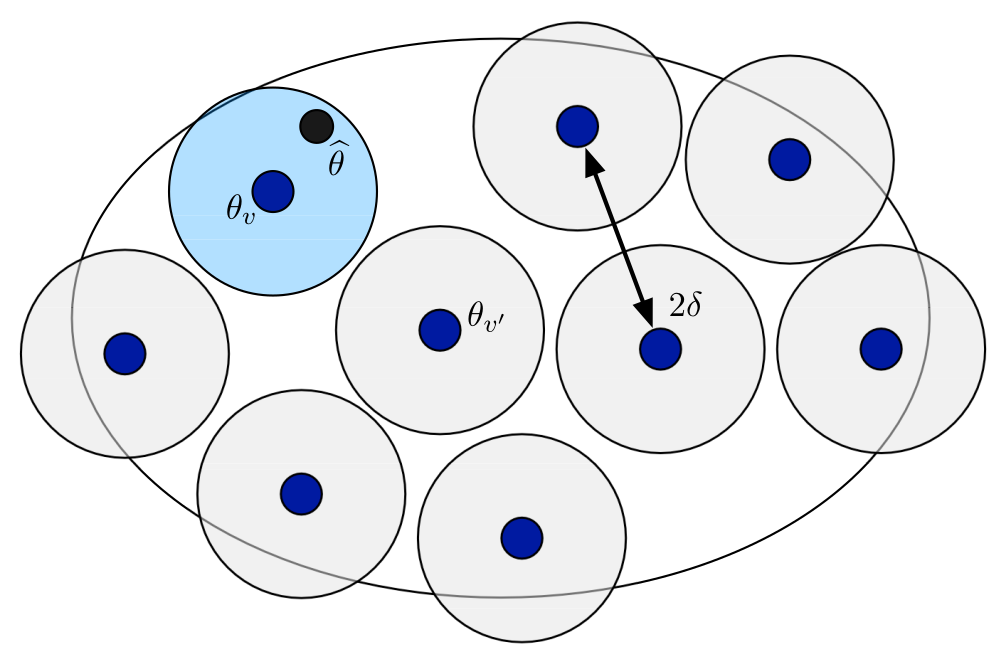
\includegraphics[width=0.5\textwidth]{figures/packing-set.png}
        \caption{From Dr.John Duchi's notes}
    \end{figure}
\item 
    % Then,
    % (what about $\sup_{v \in \mathcal{V}}$?)

    Recall $\Psi(X_1^{n}) := \argmin_{v \in \mathcal{V}} \rho(\theta_v, \widehat{\theta}(X_1^{n}))$.

    Since $\Psi(\widetilde{X}_1^{n}) \neq v \Rightarrow \rho(\theta_v, \widehat{\theta}) \geq \delta$,
    \[
    \Rightarrow \quad \mathbb{P}(\rho(\theta_v, \widehat{\theta}) \geq \delta) \geq \mathbb{P}(\Psi(\widetilde{X}_1^{n}) \neq v)
    \] 
    \end{enumerate}
\end{frame}

\begin{frame}
    Hence,
    \begin{align*}
    \sup_{P \in \mathcal{P}} \mathbb{P}(\rho(\theta, \widehat{\theta}) \geq \delta) 
    &\geq \dfrac{1}{\abs{\mathcal{V}}} \sum_{v}  \mathbb{P}(\rho(\theta_v, \widehat{\theta}) \geq \delta) \\
    &\geq \dfrac{1}{\abs{\mathcal{V}}} \sum_{v}  \mathbb{P}(\Psi(\widetilde{X}_1^{n}) \neq v) \\
    &= \mathbb{P}(\Psi(\widetilde{X}_1^{n}) \neq V)
    \end{align*} 
    \[
    \Rightarrow \inf_{\widehat{\theta}} \sup_{P \in \mathcal{P}} \; \mathbb{P}(\rho(\theta, \widehat{\theta}) \geq \delta) 
    \geq \inf_{\Psi} \mathbb{P}(\Psi(\widetilde{X}_1^{n}) \neq V)
    \] 
    \[
    \Rightarrow \mathcal{M}_n(\theta(\mathcal{P}), \Phi \circ \rho) \geq \Phi(\delta) \inf_{\Psi} \mathbb{P}(\Psi(\widetilde{X}_1^{n}) \neq V)
    \] 
\end{frame}


\begin{frame}
    \frametitle{Local Fano}
    \begin{lemma}[Derived from Fano inequality]
        \[
        \inf_{\Psi} \mathbb{P}(\Psi(\widetilde{X}_1^{n}) \neq V) \geq 1-\dfrac{I(V; \widetilde{X}_1^{n}) + \log 2}{\log \abs{\mathcal{V}}}
        \] 
    \end{lemma}
    Hence,
    \[
    \mathcal{M}_n(\theta(\mathcal{P}), \Phi \circ \rho) \geq \phi(\delta)  \left( 1 - \dfrac{I(V; \widetilde{X}_1^{n}) + \log 2}{\log \abs{\mathcal{V}}} \right)
    \] 
    % \begin{lemma}[Mutual Information to KL]
    %     \[
    %     I(V; X) \leq \dfrac{1}{\abs{V}^2} \sum_{v, v'}  D_{\rm kl}(P_v || P_{v'})
    %     \] 
    % \end{lemma}
\end{frame}
\begin{frame}
    \frametitle{Mutual Information to KL}
        % \item $D_{\rm kl} (P || Q) = D_{\rm kl}(P_1 \times \ldots P_n || Q_1 \times \ldots  \times Q_n) = \sum^{n}_{i=1} D_{\rm kl}(P_i|| Q_i) $ for $P, Q$ are product of independent RVs.
        For $X_1^{n} \sim P_v, v \sim \text{Uni}(\mathcal{V})$. 
        Define
        \[
        \overline{P} = \dfrac{1}{\abs{\mathcal{V}}} \sum_{v}  P_v
        \] 
        then
        \begin{align*}
        I(V; X_1^{n}) = D_{\rm kl} \left(  \mathbb{P}_{(V, X_1^{n})} || \mathbb{P}_V \mathbb{P}_{X_{1}^{n}}\right)
        &= \sum_{v} \sum_{X_1^{n}} \mathbb{P}(v, x_{1}^{n}) \log \dfrac{ \mathbb{P} (v, x_1^{n})}{ \mathbb{P}(v) \mathbb{P}(x_1^{n})} \\
        &= \sum_{v} \mathbb{P}(v) \sum_{X_1^{n}} \mathbb{P}(x_{1}^{n} | v) \log \dfrac{ \mathbb{P} (x_1^{n}|v)}{ \mathbb{P}(x_1^{n})} \\
        &= \sum_{v} \mathbb{P}(v) D_{\rm kl} \left( P_v || \overline{P} \right) \\
        &=\dfrac{1}{\abs{\mathcal{V}}} \sum_{v} D_{\rm kl} (P_v || \overline{P}) \\
        &\leq \dfrac{1}{\abs{\mathcal{V}}^2} \sum_{v, v'} D_{\rm kl} (P_v || P_{v'})  \text{(concavity of $\log$)}
        \end{align*} 

        % And then, weakening \ldots 
        % \begin{align*}
        % \dfrac{1}{\abs{\mathcal{V}}} \sum_{v} D_{\rm kl} (P_v || \overline{P}) 
        % \end{align*}
        
    \end{frame}

\begin{frame}
    \frametitle{How to use: A Recipe}
    \begin{align}
    &\mathcal{M}_n(\theta(\mathcal{P}), \Phi \circ \rho) \geq \phi(\delta) \left( 1 - \dfrac{I(V; \widetilde{X}_1^{n}) + \log 2}{\log \abs{\mathcal{V}}} \right) \label{eq:1} \\ 
    &I(V; \widetilde{\mathcal{X}}_1^{n}) \leq \dfrac{1}{\abs{\mathcal{V}}^2} \sum_{v, v' \in \mathcal{V}} D_{\rm kl}(P_v || D_{v'}) \label{eq:2}
    \end{align} 
    \begin{itemize} 
        \item Construct a packing set $\set{\theta_v| v\in \mathcal{V}}$ and then apply inequality  \eqref{eq:1}
            \begin{itemize}
                \item It needs to satisfy $D_{\rm kl}(P_v ||P_{v'}) \leq f(\delta)$ for some $f$
                \item And $\abs{\mathcal{V}}$ need to be large.
            \end{itemize}
        \item Compute the bound $I(V; \widetilde{X}_1^{n})$ as a function of $\delta$ using \eqref{eq:2}
        \item Choose an optimal $\delta$
    \end{itemize}
\end{frame}


\begin{frame}
    \frametitle{How to use: Example}
    \textbf{Example. }
    Given the family $\mathcal{N}_d =\set{N(\theta; \sigma^2 I_d) \mid \theta \in \mathbb{R}^{d}}$. The task is to estimate the mean $\theta(P)$ for some $P \in \mathcal{N}_n$ given $X_1^{n}$ samples drawn i.i.d from $P$. We wish to find out the lower bound of minimax error in term of mean-squared error. 

    \textbf{Solution.}
    Let's construct the local packing set $\set{\theta_v | v \in \mathcal{V}}$:

    \begin{itemize}
        \item Let $\mathcal{V}$ be a $1/2$-packing of unit  $\ell_2$-ball where $\abs{\mathcal{V}} \geq 2^{d}$. It is guaranteed that such $\mathcal{V}$ exists.
        \item Then our $\delta/2$-packing set is $\set{\delta v \in \mathbb{R}^{d} | v \in \mathcal{V}}$, since
    \[
    \norm{\theta_v - \theta_{v'}}_2 = \delta \norm{v - v'}_2 \geq \dfrac{\delta}{2} \quad \text{(since $\mathcal{V}$ is a 1/2-packing set)}
    \] 
    \end{itemize}
    Apply our bound,
    \begin{align*}
        \mathcal{M}_n(\theta(\mathcal{N}_d), \norm{\cdot}^2) 
        &\geq \Psi(\delta) \left( 1- \dfrac{I(V; X_1^{n}) +\log 2}{ \log \abs{\mathcal{V}}} \right)\\
        &\geq \left( \dfrac{1}{2} \dfrac{\delta}{2} \right)^2 \left( 1- \dfrac{I(V;X_1^{n}) + \log 2}{\log \abs{\mathcal{V}}} \right) \\
        &= \dfrac{\delta^2}{16} \left( 1- \dfrac{I(V;X_1^{n}) + \log 2}{\log \abs{\mathcal{V}}} \right)
    \end{align*}
\end{frame}

\begin{frame}
    And,
\begin{align*}
    I(V; X_1^{n}) 
    &\leq \dfrac{1}{\abs{\mathcal{V}}^2} \sum_{v, v'}  D_{\rm kl}(P_v^{n} || P_{v'}^{n})   \\
    &= \dfrac{1}{\abs{\mathcal{V}}^2} \sum_{v, v'} n D_{\rm kl}\left( N(\delta v, \sigma^2 I_d), N(\delta v', \sigma^2 I_d) \right) \\
    &= n D_{\rm kl}\left( N(\delta v, \sigma^2 I_d), N(\delta v', \sigma^2 I_d) \right) \\
    &= n \dfrac{\delta^2}{2\sigma^2 } \norm{v - v'}^2 
    \leq \dfrac{n \delta^2}{2 \sigma^2}
\end{align*}
    
Let's combine these 2 inequalities above,
\begin{align*}
    \mathcal{M}_n(\theta(\mathcal{N}_d), \norm{\cdot}^2) 
    &\geq \dfrac{\delta^2}{16} \left( 1 - \dfrac{\dfrac{n \delta^2}{2 \sigma^2} + \log 2}{d \log 2} \right)
    % = \dfrac{1}{32 d \sigma^2 \log 2} \left(  \delta^2 (2 \sigma^2 (d-1) \log 2 - n\delta^2)\right)
\end{align*} 
That bound's optimal value is achieved at $\delta^2 = \dfrac{(d-1)\sigma^2 \log 2}{n}$, and the optimal value is
\[
\dfrac{(d-1)^2 \sigma^2 \log 2}{32 dn} \Rightarrow O\left(  \dfrac{d\sigma^2}{n} \right)
\] 
\end{frame}

\begin{frame}
    \frametitle{Proof of the claim on packing number}
\textit{Claim:} There exists a $1/2$-packing set of unit $\ell_2$-ball with cardinality at least $2^{d}$.

\textit{Proof:}
    \begin{itemize}
        \item A $\delta$-packing of the set $\Theta$ with respect to $\rho$ is a set 
    $\set{\theta_1, \ldots , \theta_M}, \theta_i \in \Theta, i=1,\ldots , N$ such that $\rho(\theta_v, \theta_{v'}) \geq \delta \; \forall v \neq v'$.
    \item Then $\delta$-packing number is 
    \[
    M(\delta, \Theta, \rho) = \sup \set{M \in \mathbb{N}: \text{there exists a $\delta$-packing $\set{\theta_1, \ldots , \theta_M}$ of $\Theta$ }}
    \] 

    \end{itemize}
    We have 
    \[
    \begin{cases}
        &M(\delta, \Theta, \rho) \geq N(\delta, \Theta, \rho) \\
        &N(\delta, \mathbb{B}, \norm{\cdot}) \geq (1/\delta)^{d}
    \end{cases}
    \Rightarrow 
   M(1/2, \mathbb{B}, \norm{\cdot}) \geq 2^{d}
    \] 
    \begin{itemize}
        \item For the first inequality, denote $\widehat{\Theta}$ be a $\delta$-packing of $\Theta$ with size of $M(\delta, \Theta, \rho)$.  Since there is no $\theta \in \Theta$ we can add to $\widehat{\Theta}$ such that $\rho(\theta, \widehat{\theta}) \geq \delta$, $ \widehat{\Theta}$ is also a $\delta$-covering of $\Theta$.
        \item For the second inequality, let $\set{v_1, \ldots , v_N}$ as a $\delta$-covering of $\mathbb{B}$, then
            \[
            \text{Vol}(\mathbb{B}(\bm{0}, 1)) \leq \sum^{N}_{i=1} \text{Vol}(\mathbb{B}(v_i, \delta))
            = N \text{Vol}(\mathbb{B}(v_1, \delta)) = N \delta^{d} \text{Vol}(\mathbb{B}(\bm{0}, 1))
            \] 
    \end{itemize}
\end{frame}

\begin{frame}
    \frametitle{Proof of the bound on mutual information}
    \begin{proposition}[Fano inequality]
        For any Markov chain $V \rightarrow X \rightarrow \widehat{V}$, we have
        \[
        h_2( \mathbb{P}(\widehat{V} \neq V)) + \mathbb{P}(\widehat{V} \neq V) \log (\abs{\mathcal{V}} - 1) \geq H(V|\widehat{V})
        \] 
        where $h_2(p) = -p \log(p) - (1-p)\log(1-p)$ is entropy of a Bernoulli RV with parameter $p$.
    \end{proposition}
    Apply this proposition for $V$ being a uniform RV over  $\mathcal{V}$,
    \begin{align*}
    H(V | \widehat{V}) = H(V) - I(V;\widehat{V}) 
    = \log \abs{\mathcal{V}} - I(V; \widehat{V}) 
    \geq \log \abs{\mathcal{V}} - I(V; X)
    \end{align*}
    Hence,
    \begin{align*}
    \log 2 + \mathbb{P}(V \neq \widehat{V}) \log(\abs{\mathcal{V}}) 
    &> \log h_2( \mathbb{P}(V \neq \widehat{V})) + \mathbb{P}(V \neq \widehat{V}) \log(\abs{\mathcal{V}}-1) \\
    &\geq H(V|\widehat{V})  \\
    &\geq \log \abs{\mathcal{V}} - I(V; X) \\
    \end{align*} 
    \[
    \Rightarrow
    \mathbb{P}(V \neq \widehat{V}) \geq 1- \dfrac{I(V;X) + \log2}{\log \abs{\mathcal{V}}}
    \] 
    
    % \begin{corollary}
    %     Assume $V$ is uniform on  $\mathcal{V}$. For any Markov chain $V \rightarrow X \rightarrow \widehat{V}$, we have
    %     \[
    %     \mathbb{P}(\widehat{V} \neq V) \geq 1- \dfrac{I(V; X) + \log 2}{\log \abs{\mathcal{V}}}
    %     \] 
    % \end{corollary}
\end{frame}
\begin{frame}
    \frametitle{Proof of Fano Inequality}
    Let $E=1$ be the event  $V \neq \widehat{V}$, $E=0$ otherwise.
    We have
    \begin{align*}
        H(V, E|\widehat{V}) 
        &= H(V| E, \widehat{V}) + H(E |\widehat{V}) \quad \text{(chain rule)} \\
        &= \mathbb{P}(E=1) H(V| E=1, \widehat{V}) + \mathbb{P}(E=0)  H(V|E=0, \widehat{V}) + H(E| \widehat{V}) \\
        &= \mathbb{P}(E=1) H(V|E=1, \widehat{V}) + H(E|\widehat{V})
    \end{align*}
    We also have
    \begin{align*}
        H(V, E|\widehat{V}) 
        &= H(E|V, \widehat{V}) + H(V|\widehat{V}) \\
        &= H(V|\widehat{V})
    \end{align*}
    Hence,
    \begin{align*}
    H(V|\widehat{V}) 
    &= \mathbb{P}(E=1) H(V|E=1, \widehat{V}) + H(E|\widehat{V}) \\
    &\leq \mathbb{P}(E=1) \log \abs{\mathcal{V}-1} + H(E) \\
    &= \mathbb{P}(V \neq \widehat{V}) \log (\abs{\mathcal{V}}-1) + h_2( \mathbb{P}(V \neq \widehat{V})) \\
    \end{align*}
    
\end{frame}

\begin{frame}
    \frametitle{A variant: Distance-based Fano method}
    The previous derivation requires a construction of a packing set to translate to a hypothesis testing error.
    \[
        \mathcal{M}_n(\theta(\mathcal{P}), \Phi \circ \rho) \geq \Phi(\delta) \inf_{\Psi} \mathbb{P}(\Psi(\widetilde{X}_1^{n}) \neq V)
    \] 
    The main reason is (derived) Fano's inequality:
    \[
    \mathbb{P}(\widehat{V} \neq V) \geq 1 - \dfrac{I(V; X_1^{n}) + \log 2}{ \log \abs{\mathcal{V}}}
    \] 
    We can bound minimax without explicitly constructing packing set.
    \[
    \mathbb{P}(\rho_{\mathcal{V}}(\widehat{V}, V) > t) \geq 1 - \dfrac{I(V;X_1^{n}) + \log 2}{\log (\abs{\mathcal{V}}/N_t^{\max})}
    \] 
    % where
    % \[
    % N_t^{\max} := \max_{v \in \mathcal{V}} \set{\text{card}\set{v' \in \mathcal{V} | \rho_{\mathcal{V}}(v, v') \leq t}}
    % \] 
    Then,
    \[
    \mathcal{M}_n(\theta(\mathcal{P}), \Phi \circ \rho) \geq \Phi \left( \dfrac{\delta(t)}{2} \right) \left[ 1-\dfrac{I(X; V) + \log 2}{\log \dfrac{\abs{\mathcal{V}}}{N_t^{\max}}} \right]
    \] 
    where 
            \[
            \delta(t) := \sup \set{\delta | \rho(\theta_v, \theta_{v'}) \geq \delta \quad \text{for all } v, v'\in \mathcal{V} \text{ such that } \rho_{\mathcal{V}}(v, v') > t}
            \] 
\end{frame}

\begin{frame}
    \frametitle{Intentional Blank}
\end{frame}

\begin{frame}
    \frametitle{Setting}
    \begin{itemize}
        \item From a distribution family $\mathcal{P} = {\blue \mathcal{N}_d = \set{N(\theta, I_d) | \theta \in \mathbb{R}^{d}}}$, God chooses a distribution $P \in \mathcal{P}$.
        \item A set of $n$ i.i.d samples $X_1^{n}$ are drawn from  $P$.
        \item Task: estimating $\theta(P)$ from given samples. 
        \item Quality of estimator $\widehat{\theta}$ is measured by $\Phi(\rho(\theta, \widehat{\theta})) {\blue = \norm{\theta - \widehat{\theta}}^2}$, where:
            \begin{itemize}
                \item $\theta = \theta(P)$  is {\blue expectation} of $P = {\blue N(\theta, I_d)}$
                \item  $\widehat{\theta} = \widehat{\theta}(X_1^{n})$ is the estimator of interest. Examples: $n^{-1}(\sum^{n}_{i=1} X_i )$, $X_1$.
                \item $\Phi(t)  {\blue = t^2}$ is a non-decreasing function
                \item $\rho(\theta, \widehat{\theta}) {\blue = \norm{\theta - \widehat{\theta}}}$ is a semimetric
            \end{itemize}
        \item Question: What would be the best performance of an ideal estimator in the worse case?
    \end{itemize}
    \[
    \mathcal{M}_n(\theta(\mathcal{P}), \Phi \circ \rho) := \inf_{\widehat{\theta}} \sup_{P \in \mathcal{P}} \mathbb{E} \left[  \Phi(\rho(\theta, \widehat{\theta})) \right]
    \] 
    Finding exact $\mathcal{M}()$ is difficult, instead our attempt is to find a lower bound of it.
    % WHY, MOTIVATION?
\end{frame}


% \begin{frame}
%     \frametitle{Let's start with an example}
%     \begin{itemize}
%         \item Given a family of Gaussian $\mathcal{N}_d = \set{N(\theta, \sigma^2 I_d) | \theta \in \mathbb{R}^{d}}$.
%         \item God chooses a distribution $P \in \mathcal{N}_d$.
%         \item A set of $n$ i.i.d samples are drawn from  $P$. 
%         \item Task: estimate the mean $\theta$ from $n$ samples.
%         \item Quality of estimator is measured by $ \mathbb{E}\left[  \norm{\theta - \widehat{\theta}}^2\right]$
%     \end{itemize}
% What could be the best performance in the worse case scenario?
% \begin{itemize}
%     \item If $d=1$, we can use Cramer-Rao lower bound.
%     \item Sample mean estimator have the error of  $\dfrac{d\sigma^2}{n}$, let's see if this error can be improved.
% \end{itemize}
% \end{frame}

\begin{frame}
\frametitle{General Approach to Find Lower Bound}   

    \[
    \mathcal{M}_n(\theta(\mathcal{P}), \Phi \circ \rho) := \inf_{\widehat{\theta}} \sup_{P \in \mathcal{P}} \mathbb{E} \left[  \Phi(\rho(\theta, \widehat{\theta})) \right]
    \] 
    \begin{enumerate}
        \item Translate to probability
            \[
            \inf_{\widehat{\theta}} \sup_{P \in \mathcal{P}} \mathbb{E} \left[  \Phi(\rho(\theta, \widehat{\theta})) \right]
            \geq \Phi(\delta) \inf_{\widehat{\theta}} \sup_{P \in \mathcal{P}} \mathbb{P}(\rho(\theta, \widehat{\theta}) \geq \delta)
            \] 
        \item Reduce the whole space $ \mathcal{P}$ to a finite set $\set{\theta_v| v \in \mathcal{V}}$
            \[
            \sup_{P \in \mathcal{P}} \sum_{v \in \mathcal{V}} \mathbb{P}(\rho(\theta, \widehat{\theta}) \geq \delta) \geq \dfrac{1}{\abs{\mathcal{V}}} \mathbb{P}(\rho(\theta_v, \widehat{\theta}) \geq \delta)
            \] 
        \item Reduce to a hypothesis testing error. For $V \sim \mathcal{U}(\mathcal{V})$ (required $\mathcal{V}$ to have some properties)
            \[
            \mathbb{P}(\rho(\theta_V, \widehat{\theta}) \geq \delta) \geq \mathbb{P}(\Psi(X_1^{n}) \neq V)
            \] 
        \item Finding concrete bound based on specific problems.

    \end{enumerate}
\end{frame}
\begin{frame}
    \frametitle{How to use: A Recipe}
    \begin{equation}
    \label{eq:11}
    \mathcal{M}_n(\theta(\mathcal{P}), \Phi \circ \rho) \geq \Phi(\delta) \left( 1 - \dfrac{I(V; \widetilde{X}_1^{n}) + \log 2}{\log \abs{\mathcal{V}}} \right) 
    \end{equation}

    \begin{equation}
\label{eq:22}
    I(V; \widetilde{\mathcal{X}}_1^{n}) \leq \dfrac{1}{\abs{\mathcal{V}}^2} \sum_{v, v' \in \mathcal{V}} D_{\rm kl}(P_v || D_{v'}) 
    \end{equation}

    \begin{itemize} 
        \item Construct a packing set $\set{\theta_v| v\in \mathcal{V}}$. 
            \begin{itemize}
                \item And $\abs{\mathcal{V}}$ need to be large.
                \item Example: $\abs{\mathcal{V}} \geq 2^{d}$
            \end{itemize}

        \item Evaluate or upper bound $D_{\rm kl} (P_v || P_{v'})$.
            \begin{itemize}
                \item Example: $I(V; \widetilde{X}_1^{n}) \leq O(n \delta^2)$
            \end{itemize}
    \end{itemize}
\end{frame}

\begin{frame}
    % \begin{itemize}
        % \item A $\delta$-packing set $\set{\theta_1, \ldots , \theta_n}$ respect to $\rho$ is a set such that
        %     \[
        %     \rho(\theta_i, \theta_j) \geq \delta \quad \forall i \neq j
        %     \] 
    % \end{itemize}
    \begin{theorem}
        Assume that there exist $\set{P_v \in \mathcal{P}| v\in \mathcal{V}}, \abs{\mathcal{V}} \leq \infty$ such that for $v \neq v'$,  $\rho(\theta(P_v), \theta(P_{v'})) \geq 2\delta$.
        Define
        \begin{itemize}
            \item $V$ to be a RV with uniform distribution over  $\mathcal{V}$, and given $V=v$ we draw $\widetilde{X}_1^{n} \sim P_v$.
            \item For an estimator $\widehat{\theta}$, let $\Psi(X_1^{n}) := \argmin_{v \in \mathcal{V}} \rho(\theta(P_v), \widehat{\theta}(X_1^{n}))$
        \end{itemize}
        Then,
        \[
        \mathcal{M}_n(\theta(\mathcal{P}), \Phi \circ \rho) \geq \Phi(\delta) \inf_{\Psi} \mathbb{P}(\Psi(\widetilde{X}_1^{n}) \neq V)
        \] 
    \end{theorem}
    \begin{lemma}[Derived from Fano inequality]
        \[
        \inf_{\Psi} \mathbb{P}(\Psi(\widetilde{X}_1^{n}) \neq V) \geq 1-\dfrac{I(V; \widetilde{X}_1^{n}) + \log 2}{\log \abs{\mathcal{V}}}
        \] 
    \end{lemma}
    Some remarks:
    \begin{itemize}
        % \item This theorem bounds the minimax risk via a hypothesis testing error.
        \item The $X_1^{n}$ in the RHS is different from the $\widetilde{X}_1^{n}$ in the LHS. $\widetilde{X}_1^{n}$ are never observed and only served for our analysis.
        \item Choosing $\delta$ to obtain optimal lower bound. 
            % Moreover, it is just a pseudo-data which we never actually ``touch'' it.
        % \item In the following, $\theta_v := \theta(P_v)$, and dependence on $\widetilde{X}_1^{n}$ might be omitted.
    \end{itemize}
\end{frame}

\begin{frame}
    \frametitle{Local Fano}
    \begin{lemma}[Derived from Fano inequality]
        \[
        \inf_{\Psi} \mathbb{P}(\Psi(\widetilde{X}_1^{n}) \neq V) \geq 1-\dfrac{I(V; \widetilde{X}_1^{n}) + \log 2}{\log \abs{\mathcal{V}}}
        \] 
    \end{lemma}
    Hence,
    \[
    \mathcal{M}_n(\theta(\mathcal{P}), \Phi \circ \rho) \geq \phi(\delta)  \left( 1 - \dfrac{I(V; \widetilde{X}_1^{n}) + \log 2}{\log \abs{\mathcal{V}}} \right)
    \] 
    % \begin{lemma}[Mutual Information to KL]
    %     \[
    %     I(V; X) \leq \dfrac{1}{\abs{V}^2} \sum_{v, v'}  D_{\rm kl}(P_v || P_{v'})
    %     \] 
    % \end{lemma}
\end{frame}

\end{document}
